% !TEX root = ../main.tex
\chapter{Temporal Difference Learning}
TD learning is a model-free reinforcement learning method that learns by bootstrapping and for this reason also work for incomplete episodes. 

\section{Limits of Monte Carlo approaches}
MC only works on episodic tasks (however considering the $\gamma$-discounted return, it can be applied to continuing tasks as well). Moreover MC does not exploit available information as soon as it is collected, so we are not using the rewards as soon as they are available.

\section{Monte Carlo vs TD-Learning}

MC methods wait for the actual value of the return $G_t$ to update the estimation of $v(\pi)$.
\[V(S_t)\leftarrow V(S_t) + \alpha [G_t - V(S_t)]\]

TD methods, on the other hand, update the estimation of $v(\pi)$ after each step, using the immediate reward and the estimated value of the next state.
\[V(S_t)\leftarrow V(S_t) + \alpha [R_{t+1} + \gamma V(S_{t+1}) - V(S_t)]\]
The TD target can be seen as the best estimation of $G_t$ at time $t+1$:
\[G_t=R_{t+1}+\gamma G_{t+1}\approx R_{t+1}+\gamma\ V(S_{t+1})\]


\begin{algobox}{Tabular TD(0) for estimating $v_\pi$}
\raggedright
Input: the policy $\pi$ to be evaluated\\
Algorithm parameter: step size $\alpha \in (0,1]$

\medskip
Initialize $V(s)$, for all $s \in \mathcal{S}^+$, arbitrarily except that $V(\text{terminal}) = 0$

\medskip
Loop for each episode:\\
\hspace*{1.5em}Initialize $S$\\
\hspace*{1.5em}Loop for each step of episode:\\
\hspace*{3em}$A \leftarrow$ action given by $\pi$ for $S$\\
\hspace*{3em}Take action $A$, observe $R, S'$\\
\hspace*{3em}$V(S) \leftarrow V(S) + \alpha \bigl[R + \gamma V(S') - V(S)\bigr]$\\
\hspace*{3em}$S \leftarrow S'$\\
\hspace*{1.5em}until $S$ is terminal
\end{algobox}
TD methods still converge to the right estimation of $v_\pi$ and, typically, are faster than MC methods.

\begin{figure}[htbp]
    \centering
    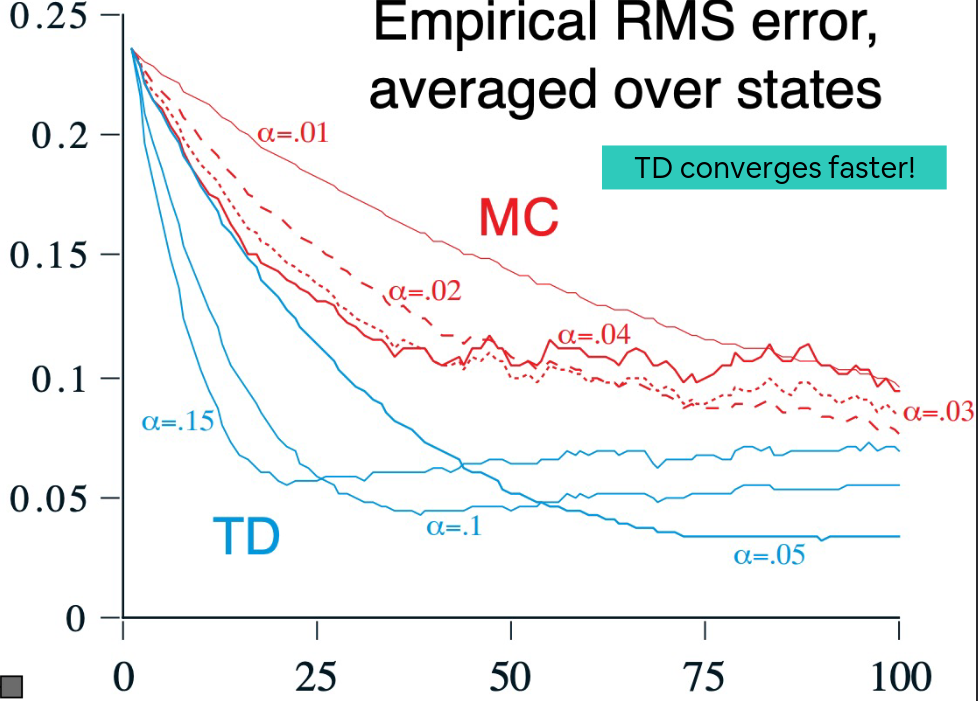
\includegraphics[width=0.85\textwidth]{figures/chapter6/image copy.png}
    \caption{Comparison between TD(0) and Monte Carlo (MC)
    in terms of estimation error. The Root Mean Square (RMS)
    error is averaged over the 5 states and then over 100
    independent runs. TD(0) generally converges faster
    than MC for the learning rates shown.}
    \label{fig:td_vs_mc}
\end{figure}

The lower $\alpha$, the lower the final error. On the other hand, higher $\alpha$ allows faster learning.

\section{Bias/Variance Trade-off}
The return $G_t$ is an unbiased estimate of $v_\pi(S_t)$. The true target $R_{t+1}+\gamma v_\pi(S_{t+1})$ is also an unbiased estimate of $v_\pi(S_t)$. However, the TD target $R_{t+1}+\gamma V(S_{t+1})$ is a biased estimate of $v_\pi(S_t)$, since it uses the current estimate $V(S_{t+1})$ instead of the true value $v_\pi(S_{t+1})$. The positve aspect of TD target is that it has much lower variane than the return $G_t$ since it depends on one random action, transition, reward:
\begin{itemize}
    \item MC has high variance and low bias
    \begin{enumerate}
        \item Good convergence properties;
        \item Not very sensitive to initial values;
        \item Simple to use and understand;
    \end{enumerate}
    \item TD has low variance and some bias
    \begin{enumerate}
        \item Usually more efficient than MC;
        \item TD(0) converges to $v_\pi(s)$;
        \item More sensitive to initial values;
    \end{enumerate}
\end{itemize}
In general we can state that unified view of the Reinforcement Learning:

\noindent
\underline{\textbf{Bootstrap}} (update involves an estimate)

\begin{itemize}
    \item \textcolor{red}{MC does not bootstrap}
    \item \textcolor{green!70!black}{DP bootstraps}
    \item \textcolor{green!70!black}{TD bootstraps}
\end{itemize}

\medskip

\noindent
\underline{\textbf{Sampling}} (use samples to estimate expectation)

\begin{itemize}
    \item \textcolor{green!70!black}{MC samples}
    \item \textcolor{red}{DP does not sample}
    \item \textcolor{green!70!black}{TD samples}
\end{itemize}

\section{TD-Learning Control}
We apply  the GPI (generalized policy iteration) approach (iteration between prediction and improvement) for solving control. Since we are model-free we use interactions over $q_\pi$. We start by considering the on-policy case. As in MC, also in this case we can consider approaches for dealing with exploration, like $\epsilon$-greedy.
\subsection{Control: SARSA-On-policy TD learning}
We need to consider transactions from (state,action) to (state,action), the update rule is:
\[Q(S_t,A_t)\leftarrow Q(S_t,A_t)+\alpha\left[R_{t+1}+\gamma Q(S_{t+1},A_{t+1})-Q(S_t,A_t)\right]\]
Pay attention that $A_{t+1}$ is the action taken according to the current policy $\pi$. 

\begin{figure}[htbp]
\centering
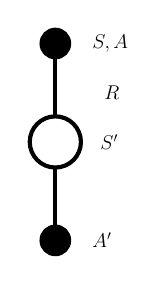
\begin{tikzpicture}[
    scale=0.5,
    transform shape,
    line width=1.5pt,
    every node/.style={font=\Large}
]

% Connections
\draw (0,0) -- (0,-5);

% Nodes
\filldraw[black] (0,0) circle (0.35);
\draw[fill=white] (0,-2.5) circle (0.65);
\filldraw[black] (0,-5) circle (0.35);

% Labels
\node[anchor=west] at (0.8,0) {$S,A$};
\node[anchor=west] at (1.1,-1.25) {$R$};
\node[anchor=west] at (1.0,-2.5) {$S'$};
\node[anchor=west] at (0.8,-5) {$A'$};

\end{tikzpicture}
\end{figure}

In the algorithm there will be the following elements:
\begin{itemize}
    \item GPI: policy evaluation + policy improvement;
    \item for loops for both episodes and steps of the episode;
    \item we will also need to consider the incremental updates (so we also need to set up an $\alpha$ parameter);
    \item for exploaration we will use $\epsilon$-greedy approach.
\end{itemize}

\begin{algobox}{Sarsa (on-policy TD control), for estimating $Q \approx q_*$}
\raggedright
Algorithm parameters: step size $\alpha \in (0,1]$, small $\varepsilon > 0$

\medskip
Initialize $Q(s,a)$, for all $s \in \mathcal{S}^+,\, a \in \mathcal{A}(s)$, arbitrarily except that $Q(\text{terminal},\cdot) = 0$

\medskip
Loop for each episode:\\
\hspace*{1.5em}Initialize $S$\\
\hspace*{1.5em}Choose $A$ from $S$ using policy derived from $Q$ (e.g., $\varepsilon$-greedy)\\
\hspace*{1.5em}Loop for each step of episode:\\
\hspace*{3em}Take action $A$, observe $R, S'$\\
\hspace*{3em}Choose $A'$ from $S'$ using policy derived from $Q$ (e.g., $\varepsilon$-greedy)\\
\hspace*{3em}$Q(S,A) \leftarrow Q(S,A) + \alpha \bigl[R + \gamma Q(S',A') - Q(S,A)\bigr]$\\
\hspace*{3em}$S \leftarrow S';\quad A \leftarrow A'$\\
\hspace*{1.5em}until $S$ is terminal
\end{algobox}
